\documentclass[11pt]{article}
\usepackage[margin=1in]{geometry}
\usepackage{times}
\usepackage{amsmath,amssymb}
\usepackage{graphicx}
\usepackage{booktabs}
\usepackage{parskip}
\usepackage{array}
\usepackage[font=small,labelfont=bf]{caption}
\usepackage{natbib}
\bibliographystyle{plainnat}
\usepackage{hyperref}
\usepackage{tikz}
\usetikzlibrary{shapes.geometric, arrows.meta, positioning}
\hypersetup{colorlinks=true, linkcolor=blue, citecolor=blue, urlcolor=blue}

\setlength{\parskip}{6pt}
\setlength{\parindent}{0pt}

\title{\textbf{The Kappa Paradox in the Room:\\Why Agreement Metrics Need to Touch GRASS}}
\author{Austin D. Semmel, Rachel Gidaro}
\date{}

\begin{document}
\maketitle
\vspace{-1cm}

\begin{abstract}
\noindent Cohen's $\kappa$, PABAK, and Gwet's AC1 use different models of chance agreement. Applied to the same data, they can place raters in different qualitative categories. The same raters can produce a $\kappa$ of 0.20 at low prevalence and 0.60 at balanced prevalence with no change in diagnostic accuracy. Through Monte Carlo simulation (6.3 million replications, 990 scenarios across 22 rater profiles), we show that fixed Landis-Koch labels correctly classify rater quality in only 43.1\% of scenarios for $\kappa$ and 73.7\% for AC1. These accuracy figures reflect the simulation grid composition and should not be interpreted as population-level estimates. No single metric with fixed labels achieves reliable classification across the prevalence spectrum. We develop GRASS (Guide for Rater Agreement under Structural Skew), a structured interpretation protocol for binary agreement metrics. GRASS consists of a four-step practitioner flowchart, a prevalence-indexed threshold table for $\kappa$, PABAK, and AC1, and a minimum reporting checklist. The present study is restricted to binary ratings from two raters under conditional independence.
\end{abstract}

%% ============================================================
\section*{Introduction}
%% ============================================================

When observed agreement between two raters is high but Cohen's $\kappa$ is low, the result is routinely described as a ``paradox'' \citep{feinstein1990high}. The behavior follows directly from the construction of the statistic. $\kappa$ corrects for chance agreement estimated from the raters' marginal distributions \citep{cohen1960coefficient}, and when prevalence is extreme, those marginals become skewed, expected agreement rises, and the chance correction grows large. The appearance of paradox arises not from the metric but from how it is interpreted. A $\kappa$ of 0.20 at prevalence 0.01 can reflect the same underlying rater accuracy as a $\kappa$ of 0.60 at prevalence 0.50, yet the first receives a ``slight'' label and the second a ``moderate'' one. The labels change; the raters do not.

The \citet{landis1977measurement} labels were introduced as informal benchmarks. They are now treated as universal standards and applied to metrics they were never designed for, including PABAK \citep{byrt1993bias}, which embeds a fundamentally different chance model. For binary outcomes, PABAK $= 2P_0 - 1$: a linear rescaling of percent agreement. Labeling a PABAK of 0.80 as ``substantial'' is equivalent to labeling 90\% agreement as ``substantial,'' without reference to whether the raters agree on rare positives, common negatives, or both. Despite decades of critique \citep{cicchetti1990high, hoehler2000bias, gwet2002kappa, sim2005kappa, vanacore2022robustness, quarfoot2016robust}, no practical guide tells a researcher how to interpret a specific $\kappa$ or PABAK value at a specific prevalence level. This study develops GRASS (Guide for Rater Agreement under Structural Skew) to fill that gap.

%% ============================================================
\section*{The GRASS Framework}
%% ============================================================

GRASS replaces the conventional workflow of computing a coefficient and applying a qualitative label with a four-step procedure that conditions on prevalence before assigning meaning to a coefficient. It produces one of three terminal outcomes: raters below threshold (study redesign needed), minority-class weakness detected (targeted intervention), or agreement adequate across both classes (proceed with full reporting). The protocol is summarized in Figure~\ref{fig:flowchart} and detailed below.

\begin{figure}[ht!]
\centering
\resizebox{0.85\textwidth}{!}{%
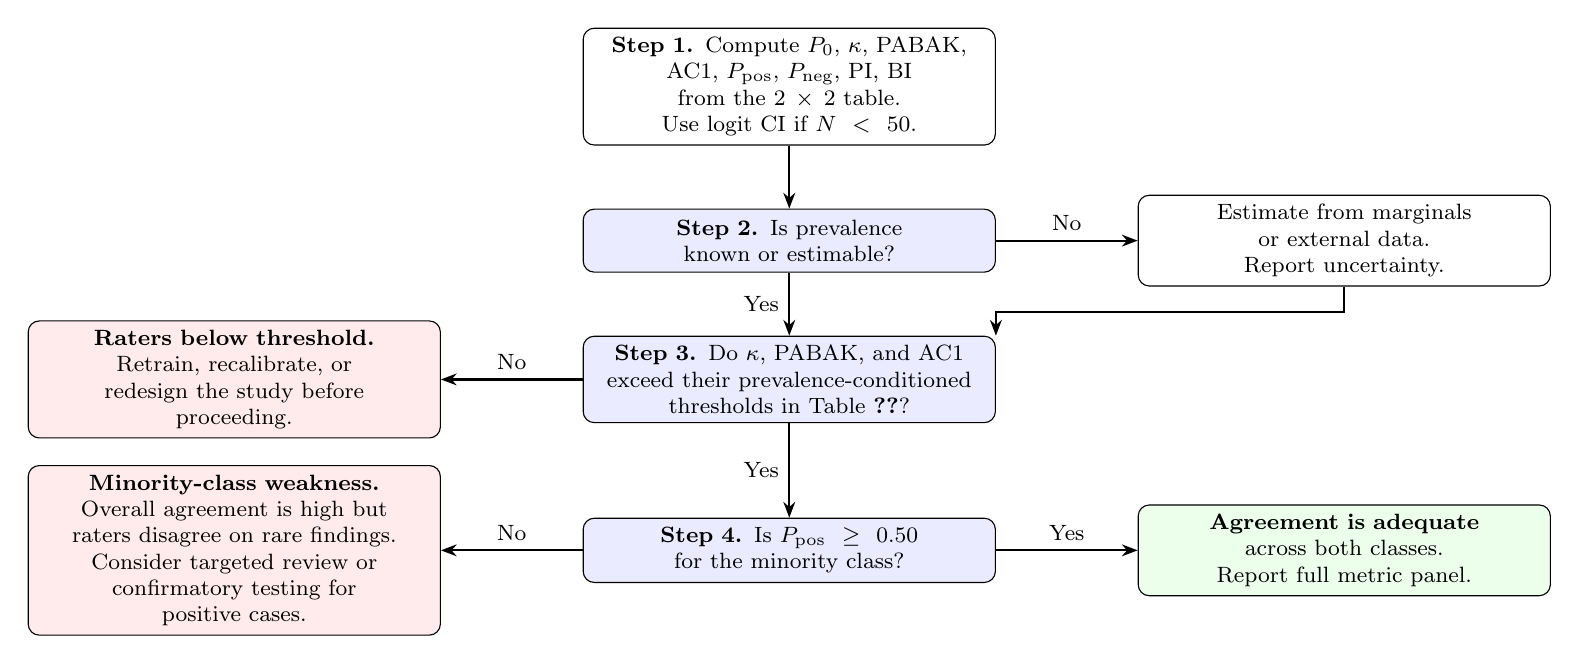
\begin{tikzpicture}[
  node distance=0.8cm,
  every node/.style={font=\footnotesize},
  block/.style={rectangle, draw, rounded corners, text width=5cm, minimum height=0.8cm, align=center},
  decision/.style={rectangle, draw, rounded corners, fill=blue!8, text width=5cm, minimum height=0.8cm, align=center},
  result/.style={rectangle, draw, fill=green!8, rounded corners, text width=5cm, minimum height=0.8cm, align=center},
  warn/.style={rectangle, draw, fill=red!8, rounded corners, text width=5cm, minimum height=0.8cm, align=center},
  arrow/.style={-{Stealth[length=2mm]}, thick}
]

% Step 1
\node[block] (start) {
  \textbf{Step 1.} Compute $P_0$, $\kappa$, PABAK,\\
  AC1, $P_{\text{pos}}$, $P_{\text{neg}}$, PI, BI\\
  from the $2\times 2$ table.\\
  Use logit CI if $N < 50$.
};

% Step 2
\node[decision, below=of start] (prev) {
  \textbf{Step 2.} Is prevalence\\known or estimable?
};

\node[block, right=1.8cm of prev] (est) {
  Estimate from marginals\\or external data.\\Report uncertainty.
};

% Step 3
\node[decision, below=of prev] (lookup) {
  \textbf{Step 3.} Do $\kappa$, PABAK, and AC1\\
  exceed their prevalence-conditioned\\
  thresholds in Table~\ref{tab:thresholds}?
};

% Step 3 outcomes
\node[warn, left=1.8cm of lookup] (fail) {
  \textbf{Raters below threshold.}\\
  Retrain, recalibrate, or\\
  redesign the study before\\
  proceeding.
};

% Step 4
\node[decision, below=1.2cm of lookup] (ppos) {
  \textbf{Step 4.} Is $P_{\text{pos}} \geq 0.50$\\
  for the minority class?
};

\node[result, right=1.8cm of ppos] (done) {
  \textbf{Agreement is adequate}\\
  across both classes.\\
  Report full metric panel.
};

\node[warn, left=1.8cm of ppos] (minority) {
  \textbf{Minority-class weakness.}\\
  Overall agreement is high but\\
  raters disagree on rare findings.\\
  Consider targeted review or\\
  confirmatory testing for\\
  positive cases.
};

% Arrows
\draw[arrow] (start) -- (prev);
\draw[arrow] (prev) -- node[above] {No} (est);
\draw[arrow] (prev) -- node[left] {Yes} (lookup);
\draw[arrow] (est.south) |- ([yshift=0.3cm]lookup.north east) -- (lookup.north east);
\draw[arrow] (lookup) -- node[left] {Yes} (ppos);
\draw[arrow] (lookup) -- node[above] {No} (fail);
\draw[arrow] (ppos) -- node[above] {Yes} (done);
\draw[arrow] (ppos) -- node[above] {No} (minority);

\end{tikzpicture}
}%
\caption{The GRASS interpretation protocol. Three terminal outcomes: raters below threshold (redesign), minority-class weakness (intervention), or agreement adequate (proceed).}
\label{fig:flowchart}
\end{figure}

\subsection*{Step 1: Compute the full metric panel}

From the $2 \times 2$ table (cells $a$, $b$, $c$, $d$ with $N$ total), compute observed agreement ($P_0 = (a+d)/N$), Cohen's $\kappa$, PABAK ($= 2P_0 - 1$), Gwet's AC1, positive agreement ($P_{\text{pos}} = 2d/(2d+b+c)$), negative agreement ($P_{\text{neg}} = 2a/(2a+b+c)$), and the prevalence and bias indices ($\text{PI} = |d-a|/N$, $\text{BI} = |b-c|/N$). Full formulas for $\kappa$ and AC1 are given in Appendix~\ref{app:algebra}. When $N < 50$ or prevalence is extreme, use the logit-transformed confidence interval for $\kappa$ rather than the standard Wald interval. The Wald interval violates $\kappa$'s $[-1,1]$ parameter bounds in 5.5\% of replications at small $N$; the logit alternative reduces this to 0.9\% (Appendix~\ref{app:ci}).

\subsection*{Step 2: Establish prevalence}

The prevalence of the target condition determines which row of the threshold table to use. If prevalence is known from the study design or an external source, use it directly. If it must be estimated from the data, report the estimate with uncertainty. The $\kappa$ threshold changes slowly in the interior of the prevalence range (0.485 at 0.20 vs.\ 0.617 at 0.50) but rapidly at the extremes (0.061 at 0.01 vs.\ 0.240 at 0.05). Prevalence estimates below 0.10 or above 0.90 should be accompanied by explicit uncertainty quantification.

\subsection*{Step 3: Look up prevalence-conditioned thresholds}

Compare $\kappa$, PABAK, and AC1 to their prevalence-conditioned thresholds in Table~\ref{tab:thresholds}. These thresholds were derived via ROC optimization across 990 simulation scenarios (Appendix~\ref{app:sim}) and identify the metric values that best separate high-quality raters ($\min(\text{Se}, \text{Sp}) \geq 0.90$) from the rest. The $\kappa$ threshold ranges from 0.061 at prevalence 0.01 to 0.617 at prevalence 0.50, a 10-fold range driven by the growth of marginal imbalance ($\Delta$) at extreme prevalence (Appendix~\ref{app:algebra}). PABAK thresholds are prevalence-stable at approximately 0.64. AC1 thresholds range from 0.640 to 0.762.

\begin{table}[h!]
\centering
\caption{Prevalence-conditioned thresholds for ``High'' quality classification ($\min(\text{Se}, \text{Sp}) \geq 0.90$). $J$ = Youden's index for the threshold. Thresholds are situational benchmarks, not fixed standards. Leave-one-profile-out stability analysis is in Table~\ref{tab:jackknife}.}
\label{tab:thresholds}
\small
\begin{tabular}{ccccccc}
\toprule
Prevalence & $\kappa$ & $J_\kappa$ & PABAK & $J_P$ & AC1 & $J_{A}$ \\
\midrule
0.01 & 0.060 & 0.88 & 0.639 & 0.93 & 0.759 & 0.83 \\
0.05 & 0.240 & 0.90 & 0.639 & 0.93 & 0.759 & 0.88 \\
0.10 & 0.385 & 0.97 & 0.636 & 0.93 & 0.740 & 0.90 \\
0.20 & 0.492 & 1.00 & 0.638 & 0.93 & 0.704 & 0.93 \\
0.50 & 0.612 & 1.00 & 0.637 & 1.00 & 0.640 & 1.00 \\
0.80 & 0.482 & 1.00 & 0.638 & 0.93 & 0.703 & 0.93 \\
0.90 & 0.376 & 0.95 & 0.638 & 0.93 & 0.730 & 0.93 \\
0.95 & 0.241 & 0.92 & 0.639 & 0.93 & 0.759 & 0.88 \\
0.99 & 0.060 & 0.88 & 0.640 & 0.93 & 0.759 & 0.83 \\
\bottomrule
\end{tabular}
\end{table}

For prevalence values between tabulated rows, linear interpolation is adequate in the interior ($0.10$--$0.90$). At the extremes ($< 0.10$ or $> 0.90$), use the nearest tabulated value.

If any metric falls below its threshold, the raters should be retrained, recalibrated, or the study redesigned before proceeding. When the three metrics disagree on whether the threshold is met, the discordance itself is informative: it signals large marginal imbalance. Report all three values, note the discordance, and let the application context determine which chance model is most relevant.

\subsection*{Step 4: Check minority-class agreement}

If the raters clear the thresholds in Step 3, check whether $P_{\text{pos}} \geq 0.50$ for the minority class. This threshold indicates that raters agree on positive cases more often than they disagree. In high-stakes applications, a stricter threshold (e.g., $P_{\text{pos}} \geq 0.70$) may be appropriate.

At very low prevalence, this gate will flag virtually all raters, including high-quality ones. For Se $=$ Sp $= 0.90$ at prevalence 0.01, the theoretical $P_{\text{pos}}$ is only 0.17 because the expected number of true positives is fewer than two per hundred subjects. In this regime, Step 4 is not diagnosing poor rater quality. It is diagnosing insufficient positive-case volume. The appropriate response is not to retrain the raters but to increase the sample size or enrich the sample for positive cases. As a rule of thumb, at least 10 expected positive cases ($N \times \text{prevalence} \geq 10$) are needed for $P_{\text{pos}}$ to be meaningfully evaluable.

\subsection*{GRASS minimum reporting standard}

Agreement studies adopting GRASS should report, at minimum:
\begin{enumerate}
\item The $2 \times 2$ table (cell counts $a, b, c, d$)
\item Prevalence index and bias index
\item $P_0$, $\kappa$, PABAK, and AC1
\item Positive and negative agreement ($P_{\text{pos}}$, $P_{\text{neg}}$)
\item 95\% confidence intervals for $\kappa$ (logit-transformed when $N < 50$ or prevalence is extreme)
\item The prevalence of the target condition
\end{enumerate}

A single coefficient with a qualitative label is not sufficient for defensible interpretation.

\subsection*{Worked example}

Two radiologists classify 200 chest films for a finding with 5\% population prevalence. The observed positive rates (7.5\% for R1, 6.5\% for R2) exceed the true prevalence because imperfect specificity produces false positives. Their $2 \times 2$ table:

\begin{table}[h!]
\centering
\begin{tabular}{lcc}
\toprule
& R2 Negative & R2 Positive \\
\midrule
R1 Negative & 180 & 5 \\
R1 Positive & 7 & 8 \\
\bottomrule
\end{tabular}
\end{table}

\noindent Computed metrics: $P_0 = 0.94$, $\kappa = 0.54$ (``moderate''), $\text{PABAK} = 0.88$ (``almost perfect''), $\text{AC1} = 0.93$, $P_{\text{pos}} = 0.57$, $P_{\text{neg}} = 0.97$, $\text{PI} = 0.86$, $\text{BI} = 0.01$.

\textbf{Step 1} produces the full metric panel. \textbf{Step 2:} prevalence is 0.05, known from the study design. \textbf{Step 3:} at prevalence 0.05, the $\kappa$ threshold is 0.240 (Table~\ref{tab:thresholds}). The observed $\kappa = 0.54$ exceeds this comfortably. PABAK (0.88) and AC1 (0.93) also exceed their thresholds (0.639 and 0.759). All three metrics pass. \textbf{Step 4:} $P_{\text{pos}} = 0.57 \geq 0.50$. The raters pass, but the margin is thin. Agreement on positive cases is modest even though overall agreement is high.

Without GRASS, Landis-Koch labels produce three different conclusions from the same data: $\kappa$ at 0.54 is ``moderate,'' PABAK at 0.88 is ``almost perfect,'' AC1 at 0.93 is ``almost perfect.'' A reviewer reading only $\kappa$ might question whether the raters are adequate. The prevalence-conditioned threshold resolves this: at 5\% prevalence, $\kappa = 0.54$ exceeds the threshold and the raters are performing well for their operating conditions. The high PI (0.86) confirms that prevalence imbalance, not poor rater quality, drives the low $\kappa$: $\Delta = 0.86^2 - 0.01^2 = 0.74$.

%% ============================================================
\section*{Findings}
%% ============================================================

The simulation underlying GRASS comprised 6.3 million replications across 990 scenarios (9 prevalence levels $\times$ 5 sample sizes $\times$ 22 rater profiles). Full design details are in Appendix~\ref{app:sim}.

\textbf{Fixed labels fail.} Applying Landis-Koch labels to $\kappa$ correctly classified rater quality in 43.1\% of scenarios (31.8\% at extreme prevalence). PABAK-based labels achieved 63.6\%. AC1 achieved the highest accuracy (73.7\%) but remains unreliable at intermediate prevalence where its adaptive chance term overcorrects. These accuracy figures reflect the simulation grid composition (7 High, 8 Medium, 7 Low profiles) and should not be interpreted as population-level estimates. The robust finding is the prevalence dependence: no metric with fixed labels produces stable classification across the prevalence spectrum.

\textbf{Three chance models, three answers.} At balanced prevalence, $\kappa$, PABAK, and AC1 converge (mean values 0.39, 0.41, 0.43). At extreme prevalence ($p = 0.01$), the same raters produce mean $\kappa = 0.07$, AC1 $= 0.51$, PABAK $= 0.41$. The divergence is governed by $\Delta = \text{PI}^2 - \text{BI}^2$ (Appendix~\ref{app:algebra}). Figure~\ref{fig:three_metrics} illustrates the separation for raters with Se $=$ Sp $= 0.90$.

\begin{figure}[h!]
\centering
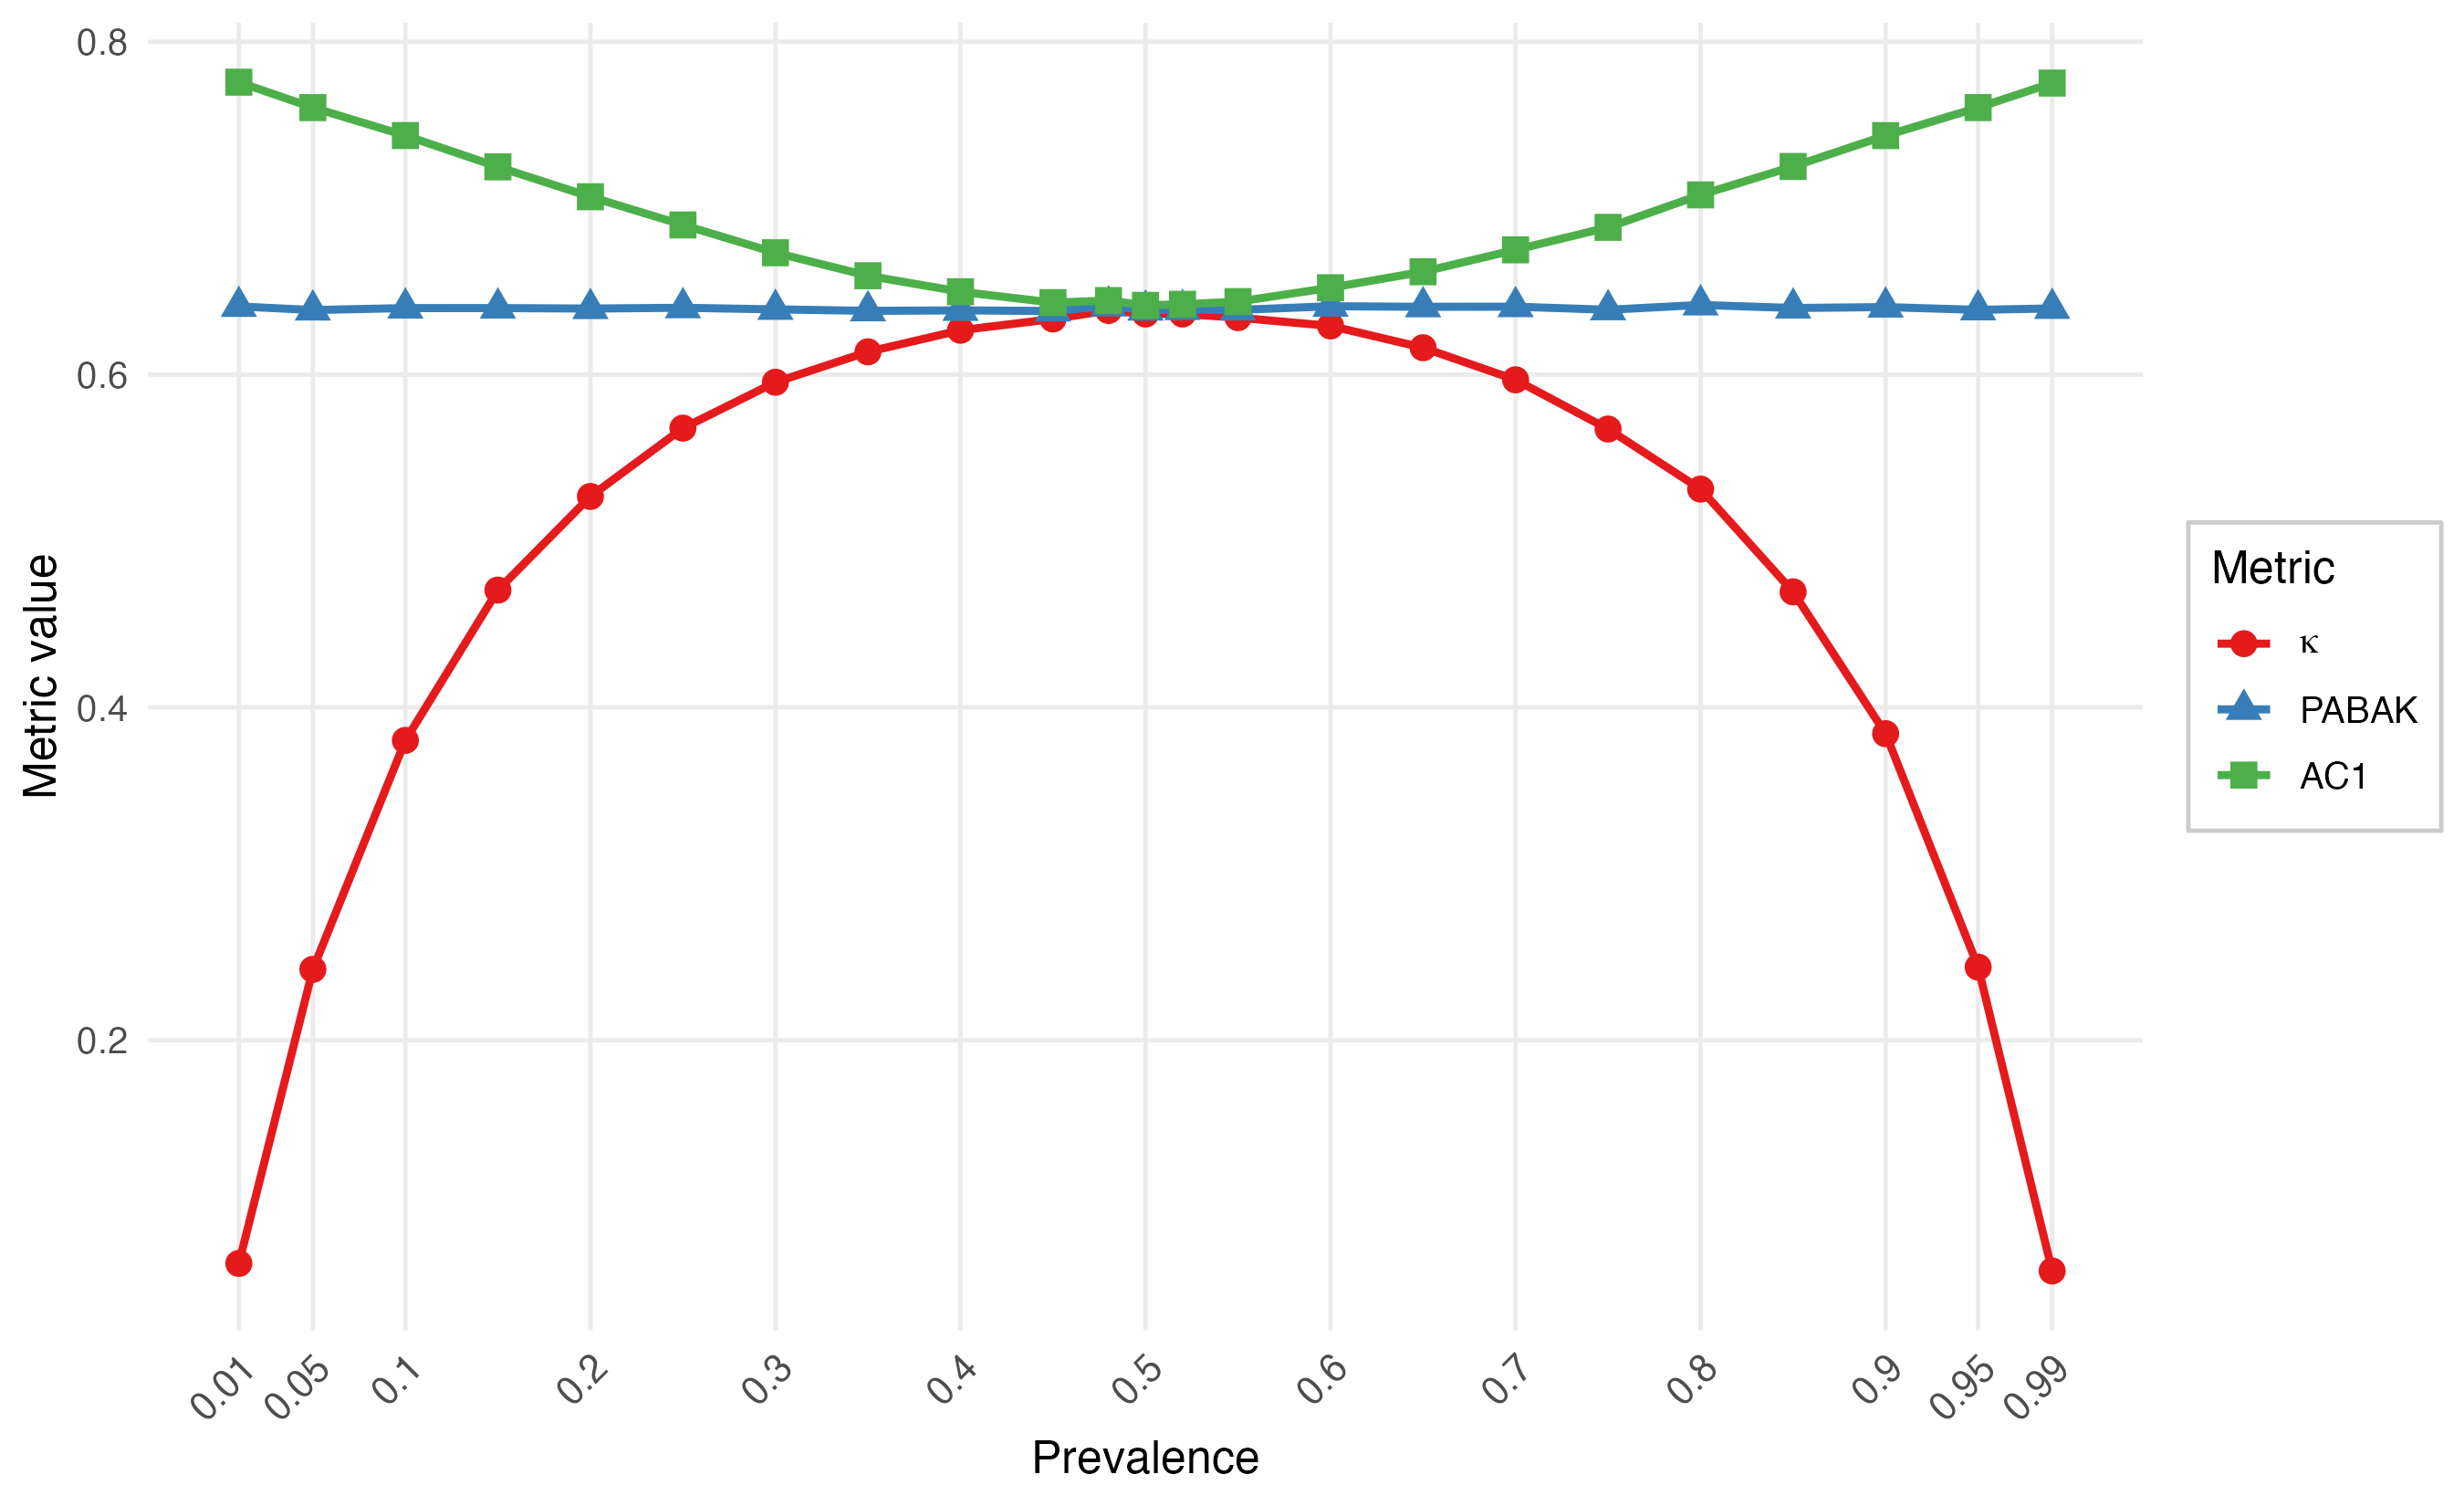
\includegraphics[width=0.85\textwidth]{figures/fig_three_metrics.png}
\caption{$\kappa$, PABAK, and AC1 for Se $=$ Sp $= 0.90$ raters ($N = 100$) across prevalence. The dashed line marks the L-K ``substantial'' threshold (0.61); $\kappa$ falls below it outside 0.20--0.80 despite unchanged rater quality.}
\label{fig:three_metrics}
\end{figure}

\textbf{Confidence intervals at the boundary.} The standard Wald CI for $\kappa$ violated the $[-1,1]$ parameter bounds in 5.5\% of replications. The logit-transformed alternative reduced this to 0.9\%. Neither method achieves nominal 95\% coverage at small $N$ and extreme prevalence (Table~\ref{tab:coverage}), but the logit interval consistently outperforms Wald by 1--3 percentage points. We recommend the logit CI as a default when $N < 50$ or prevalence is extreme. Neither method is adequate below $N = 30$ at extreme prevalence, where coverage can fall below 60\%; bootstrap CIs should be used in that regime.

%% ============================================================
\section*{Discussion}
%% ============================================================

The divergence between $\kappa$ and PABAK is governed by a single quantity: $\Delta = \text{PI}^2 - \text{BI}^2$. Prevalence imbalance drives the metrics apart. Rater bias pulls them back together. This is not new mathematics \citep{byrt1993bias}, but the GRASS framework translates it into actionable guidance. The closest precedent is the \citet{koo2016guideline} framework for intraclass correlation coefficients, which ties interpretation to study design and confidence intervals rather than fixed labels. GRASS extends this principle to categorical agreement, with prevalence as the conditioning variable.

\citet{cicchetti1990high} recommended reporting $P_{\text{pos}}$ and $P_{\text{neg}}$ alongside $\kappa$ to diagnose the paradox. This recommendation has been widely cited but inconsistently adopted. GRASS provides what was missing: prevalence-conditioned thresholds that tell practitioners what ``acceptable'' means at their prevalence level, a three-metric comparison that exposes how different chance models produce different conclusions, and a decision procedure with explicit terminal outcomes.

Prevalence-invariant alternatives exist. \citet{hoehler2000bias} proposed an adjusted $\kappa$ based on the odds ratio, which \citet{walter2001hoehler} showed is equivalent to Yule's $Y$. Adjusted $\kappa$ does not attenuate at extreme prevalence, but it is undefined when any cell count is zero and overestimates reliability when bias or prevalence effects are present. When all four cells are nonzero and the primary concern is comparing agreement across studies with different prevalence levels, adjusted $\kappa$ provides a useful prevalence-invariant benchmark. The goal of GRASS is not to propose a superior metric. It is to help practitioners interpret the metrics already in widespread use.

PABAK is prevalence-adjusted \textit{and} bias-adjusted, so a natural question is whether the GRASS thresholds should also condition on rater bias. In our simulation, prevalence alone explains 38.7\% of scenario-level $\kappa$ variation; bias explains 5.0\%. The reason is structural: PI can exceed 0.85 while BI rarely exceeds 0.20. Bias-conditioned thresholds are a natural extension but would add a second table dimension for modest incremental gain.

\subsection*{Limitations}

The profile grid contains 22 profiles (7 High, 8 Medium, 7 Low) spanning symmetric, asymmetric, and opposite-bias configurations. Leave-one-profile-out cross-validation (Table~\ref{tab:jackknife}) confirms threshold stability across the prevalence spectrum, with maximum deviation of 0.069 at balanced prevalence and $\leq 0.05$ elsewhere.

Two limitations merit attention. First, the simulation assumes conditional independence of raters given the true class. Positively correlated errors would inflate $P_0$, PABAK, and AC1, making the GRASS thresholds anti-conservative. Second, the grid covers binary 2-rater settings only; multi-class and multi-rater extensions are needed.

\subsection*{Code and data availability}

Simulation code and results are available at \url{https://github.com/defense031/grass-agreement}.

\bibliography{references}

%% ============================================================
\newpage
\appendix

\section{Algebraic Framework}
\label{app:algebra}

Consider two raters classifying $N$ subjects into binary categories. Their joint ratings produce a $2 \times 2$ table with cells $a$ (both 0), $b$ (R1=0, R2=1), $c$ (R1=1, R2=0), $d$ (both 1).

Observed agreement:
\begin{equation}
P_0 = \frac{a + d}{N}
\label{eq:p0}
\end{equation}

Cohen's $\kappa$ \citep{cohen1960coefficient}:
\begin{equation}
\kappa = \frac{P_0 - P_e}{1 - P_e}, \qquad P_e = \frac{(a+b)(a+c) + (c+d)(b+d)}{N^2}
\label{eq:kappa}
\end{equation}

PABAK \citep{byrt1993bias}:
\begin{equation}
\text{PABAK} = 2P_0 - 1
\label{eq:pabak}
\end{equation}

This is algebraically equivalent to $P_e = 0.5$. The Brennan-Prediger coefficient \citep{brennan1981coefficient} generalizes to $P_e = 1/K$.

Gwet's AC1 \citep{gwet2008computing}:
\begin{equation}
\text{AC1} = \frac{P_0 - 2\hat{p}(1-\hat{p})}{1 - 2\hat{p}(1-\hat{p})}
\label{eq:ac1}
\end{equation}
where $\hat{p}$ is the average positive rate across raters. AC1's chance term shrinks when one category dominates, producing less attenuation than $\kappa$ at extreme prevalence.

\subsection*{The divergence between $\kappa$ and PABAK}

Since $P_0 = \tfrac{1}{2}(\text{PABAK} + 1)$, substituting into (\ref{eq:kappa}) gives:
\begin{equation}
\kappa = \frac{\text{PABAK} - \Delta}{1 - \Delta}, \qquad \Delta = 2P_e - 1
\label{eq:divergence}
\end{equation}

When $\Delta = 0$ (balanced marginals), $\kappa = \text{PABAK}$. As $\Delta \to 1$, $\kappa \to 0$ regardless of $P_0$.

\citet{byrt1993bias} decomposed $P_e$ using the prevalence index PI $= |d-a|/N$ and bias index BI $= |b-c|/N$:
\begin{equation}
P_e = \frac{1}{2} + \frac{\text{PI}^2 - \text{BI}^2}{2}, \qquad \Delta = \text{PI}^2 - \text{BI}^2
\label{eq:delta_decomp}
\end{equation}

Prevalence imbalance ($\text{PI}^2$) inflates $P_e$ and attenuates $\kappa$. Rater bias ($\text{BI}^2$) acts in the opposite direction. In the typical low-prevalence study, PI is large, BI is small, $\Delta \approx \text{PI}^2$, and $\kappa$ can be severely attenuated even when $P_0$ is high.

AC1's chance term ($P_e^{\text{AC1}} = 2\hat{p}(1-\hat{p})$) does not decompose into PI and BI. It adapts to the overall category distribution, producing less attenuation than $\kappa$ at extreme prevalence but overcorrecting at intermediate prevalence.

Positive and negative agreement decompose agreement by class:
\begin{equation}
P_{\text{pos}} = \frac{2d}{2d + b + c}, \qquad P_{\text{neg}} = \frac{2a}{2a + b + c}
\label{eq:posneg}
\end{equation}

\newpage
\section{Simulation Design}
\label{app:sim}

Binary rating data were generated from a latent-class model. A true class $Y \sim \text{Bernoulli}(p)$ was drawn for each subject. Two raters produced ratings conditional on $Y$ through sensitivity and specificity parameters, with conditional independence given $Y$.

Three factors were crossed in a full factorial grid: prevalence $p \in \{0.01, 0.05, 0.10, 0.20, 0.50, 0.80, 0.90, 0.95, 0.99\}$, sample size $N \in \{10, 50, 100, 500, 1000\}$, and 22 rater profiles (Table~\ref{tab:profiles}). This produced 990 scenarios. Each received 5{,}000 replications, with stress conditions ($p \in \{0.01, 0.99\}$, $N \in \{10, 50\}$) receiving 20{,}000. Total: 6{,}270{,}000 replications. Monte Carlo standard error for $\kappa$ remained below 0.007 across all scenarios.

\begin{table}[h!]
\centering
\caption{Rater profiles with operating characteristics and ground-truth quality bands. Quality band: High if $\min(\text{Se}, \text{Sp}) \geq 0.90$, Medium if $\geq 0.70$, Low if $< 0.70$.}
\label{tab:profiles}
\small
\begin{tabular}{lcccccc}
\toprule
Profile & Se$_1$ & Sp$_1$ & Se$_2$ & Sp$_2$ & $\min$ & Band \\
\midrule
Symmetric, low accuracy         & 0.65 & 0.65 & 0.65 & 0.65 & 0.65 & Low \\
Symmetric, very low accuracy    & 0.60 & 0.60 & 0.60 & 0.60 & 0.60 & Low \\
Symmetric, moderate accuracy    & 0.75 & 0.75 & 0.75 & 0.75 & 0.75 & Medium \\
Both favor positives            & 0.95 & 0.70 & 0.95 & 0.70 & 0.70 & Medium \\
Both favor negatives            & 0.70 & 0.95 & 0.70 & 0.95 & 0.70 & Medium \\
R2 misses positives             & 0.95 & 0.90 & 0.70 & 0.90 & 0.70 & Medium \\
R2 misses negatives             & 0.90 & 0.95 & 0.90 & 0.70 & 0.70 & Medium \\
R2 worse overall                & 0.90 & 0.90 & 0.70 & 0.70 & 0.70 & Medium \\
Opposite biases (A)             & 0.90 & 0.70 & 0.70 & 0.90 & 0.70 & Medium \\
Opposite biases (B)             & 0.70 & 0.90 & 0.90 & 0.70 & 0.70 & Medium \\
Symmetric, high accuracy        & 0.90 & 0.90 & 0.90 & 0.90 & 0.90 & High \\
Symmetric, very high accuracy   & 0.95 & 0.95 & 0.95 & 0.95 & 0.95 & High \\
Symmetric, high (alt)           & 0.92 & 0.92 & 0.92 & 0.92 & 0.92 & High \\
High, Se dominant               & 0.95 & 0.90 & 0.95 & 0.90 & 0.90 & High \\
High, Sp dominant               & 0.90 & 0.95 & 0.90 & 0.95 & 0.90 & High \\
High, complementary             & 0.95 & 0.92 & 0.92 & 0.95 & 0.92 & High \\
High, R2 slightly lower         & 0.95 & 0.95 & 0.90 & 0.90 & 0.90 & High \\
Low, poor Se / good Sp          & 0.50 & 0.90 & 0.50 & 0.90 & 0.50 & Low \\
Low, good Se / poor Sp          & 0.90 & 0.50 & 0.90 & 0.50 & 0.50 & Low \\
Low, R2 worse                   & 0.65 & 0.65 & 0.50 & 0.50 & 0.50 & Low \\
Low, opposite biases            & 0.60 & 0.50 & 0.50 & 0.60 & 0.50 & Low \\
Low, symmetric very poor        & 0.55 & 0.55 & 0.55 & 0.55 & 0.55 & Low \\
\bottomrule
\end{tabular}
\end{table}

Ground-truth quality was defined via $\min(\text{Se}, \text{Sp})$ across both raters. This conservative definition flags raters whose weakest operating characteristic falls below threshold. Sensitivity analysis across strict ($\geq 0.95 / \geq 0.75$) and lenient ($\geq 0.85 / \geq 0.65$) definitions confirmed that the qualitative conclusion (prevalence-dependent thresholds) holds under all three schemes.

Prevalence-conditioned thresholds were derived by treating the classification of rater quality (High vs.\ not-High) as a binary discrimination problem. Within each prevalence stratum, the metric value maximizing Youden's $J$ (sensitivity $+$ specificity $- 1$) was selected. This was computed separately for $\kappa$, PABAK, and AC1.

\newpage
\section{Confidence Interval Analysis}
\label{app:ci}

The standard Wald CI for $\kappa$ ($\kappa \pm z_{\alpha/2} \cdot \hat{\sigma}_\kappa$) can exceed the $[-1,1]$ parameter bounds at small $N$ and extreme prevalence \citep{wilson1927probable}. We implement a logit-transformed alternative:
\begin{equation}
\kappa_{\text{logit}}^{\pm} = 2 \cdot \text{logit}^{-1}\!\left(\text{logit}(\kappa^*) \pm z_{\alpha/2} \cdot \frac{\hat{\sigma}_\kappa}{2\kappa^*(1 - \kappa^*)}\right) - 1
\label{eq:logit_ci}
\end{equation}
where $\kappa^* = (\kappa + 1)/2$. This interval is guaranteed to lie within $[-1,1]$. The logit transform inherits the reliability of $\hat{\sigma}_\kappa$; for $N < 30$ at extreme prevalence, bootstrap CIs remain the gold standard.

A naive Wilson-type approach (Wilson score interval applied to $P_0$, transformed to the $\kappa$ scale via $(\cdot - P_e)/(1-P_e)$) produces \textit{worse} boundary violations than Wald (77.5\% at $N=10$, extreme prevalence) because the small denominator $1 - P_e$ amplifies the interval width.

\begin{table}[h!]
\centering
\caption{Empirical coverage proportions (\%) for 95\% CIs of $\kappa$. W = Wald, L = Logit. Nominal coverage is 95\%.}
\label{tab:coverage}
\small
\begin{tabular}{c cc cc cc cc cc}
\toprule
& \multicolumn{2}{c}{$N = 10$} & \multicolumn{2}{c}{$N = 50$} & \multicolumn{2}{c}{$N = 100$} & \multicolumn{2}{c}{$N = 500$} & \multicolumn{2}{c}{$N = 1000$} \\
\cmidrule(lr){2-3} \cmidrule(lr){4-5} \cmidrule(lr){6-7} \cmidrule(lr){8-9} \cmidrule(lr){10-11}
Prev & W & L & W & L & W & L & W & L & W & L \\
\midrule
0.01 & 58.2 & 60.7 & 90.9 & 92.2 & 91.1 & 91.9 & 90.6 & 90.7 & 90.9 & 91.0 \\
0.05 & 67.3 & 69.3 & 87.3 & 90.0 & 89.1 & 90.1 & 89.6 & 89.8 & 89.7 & 89.8 \\
0.10 & 76.0 & 77.8 & 91.2 & 92.8 & 91.7 & 92.7 & 92.1 & 92.3 & 91.9 & 92.0 \\
0.20 & 86.7 & 88.1 & 94.6 & 95.0 & 95.0 & 95.3 & 95.1 & 95.2 & 95.2 & 95.3 \\
0.50 & 94.7 & 95.2 & 96.7 & 96.9 & 96.9 & 97.0 & 96.9 & 96.9 & 97.0 & 97.1 \\
0.80 & 86.5 & 87.9 & 94.6 & 94.9 & 94.8 & 95.1 & 95.1 & 95.2 & 95.1 & 95.2 \\
0.90 & 76.2 & 78.0 & 91.1 & 92.7 & 91.6 & 92.7 & 92.0 & 92.2 & 92.0 & 92.2 \\
0.95 & 67.2 & 69.1 & 87.5 & 90.1 & 89.0 & 90.0 & 89.7 & 89.9 & 89.6 & 89.6 \\
0.99 & 58.2 & 60.7 & 90.9 & 92.2 & 91.1 & 91.9 & 90.6 & 90.7 & 90.8 & 90.8 \\
\bottomrule
\end{tabular}
\end{table}

\newpage
\section{Stability and Sensitivity}
\label{app:stability}

\begin{table}[h!]
\centering
\caption{Leave-one-profile-out stability of $\kappa$ thresholds. Max deviation indicates how much the threshold shifts when any single profile is excluded.}
\label{tab:jackknife}
\small
\begin{tabular}{ccccc}
\toprule
Prevalence & Full threshold & JK min & JK max & Max deviation \\
\midrule
0.01 & 0.060 & 0.060 & 0.067 & 0.008 \\
0.05 & 0.240 & 0.240 & 0.267 & 0.027 \\
0.10 & 0.385 & 0.353 & 0.386 & 0.032 \\
0.20 & 0.492 & 0.492 & 0.539 & 0.048 \\
0.50 & 0.612 & 0.612 & 0.681 & 0.069 \\
0.80 & 0.482 & 0.482 & 0.532 & 0.050 \\
0.90 & 0.376 & 0.357 & 0.382 & 0.018 \\
0.95 & 0.241 & 0.241 & 0.275 & 0.034 \\
0.99 & 0.060 & 0.060 & 0.073 & 0.013 \\
\bottomrule
\end{tabular}
\vspace{4pt}

\footnotesize With 22 profiles (7 High, 8 Medium, 7 Low), thresholds are stable across the full prevalence spectrum. Maximum deviation is 0.069 at balanced prevalence and $\leq 0.05$ elsewhere.
\end{table}

Under the strict ground-truth definition (High if $\min(\text{Se}, \text{Sp}) \geq 0.95$, Medium if $\geq 0.75$), L-K $\kappa$ accuracy improved to 73.0\%, driven by class imbalance: 741 of 990 scenarios fell into the ``Low'' band. Under the lenient definition (High if $\geq 0.85$, Medium if $\geq 0.65$), accuracy dropped to 20.2\%. The qualitative conclusion is robust: the $\kappa$ threshold for a given quality level varies substantially with prevalence regardless of where the ground-truth boundary is drawn.

\end{document}
